\chapter{Review Methods for Electrical Source Reconstruction}

% \pagestyle{plain}

\label{ch:review}

At some point, cite \cite{grech2008review}.

The EEG model discussed presented on the previous can be summarized on the following matrix equation
\begin{equation}
\Y = \G\, \ppar{ \J + \nu } + \varepsilon
\label{eq:general}
\end{equation}
where the varibles encode the following elements,
\begin{itemize}
\item[$\Y \in \R^{M\times T}$] EEG measurements over time,
\item[$\J \in \R^{N\times T}$] Dipole magnitudes over time,
\item[$\G \in \R^{M\times N}$] Leadfield matrix,
\end{itemize}
%
The terms $\nu \in \R^{N\times T}, \varepsilon\in\R^{M\times T}$ represent additive noise within the true values for the dipoles and sensors, respectively. 
%
Different author have proposed different sets of assumptions for such noise terms, sme of them will be discussed later.

It was discussed how this model is constructed for $M$ EEG sensors and $N$ equivalent dipoles with known orientation; if the dipole orientation is to be determined we may consider 3 superimposed dipoles, parallel to the canonical axis, for each dipole position.
%
The cases of known and unknown dipole orientations don't change the model formulation on a significant way, and thus they will be treated as a single model.

Within the context of Electrical Source Reconstruction, the computation of the leadfield matrix is referred to as the forward problem.
%
As discussed previously, this computation implies a large number of steps: identification of tissues from anatomical MRI or similar, construction of triangulated surfaces representing anatomical regions of interest (which may be simplified), setup of a number of PDEs within the anatomical regions as geometric domain, and the numerical solution of said equations by either BEM or FEM (or a different method).

A further discussion of the forward model is beyond the scope of this work.
%
After this point, we will consider the leadfield matrix $\G$ to be given for each set of anatomical data and electrodes montage.

\section{Inverse problem formulations}

The main aim of this work will be the task of `recovering' $\J$ once the data $\Y$ and some additional assumptions are considered.

In the absence of biological noise ($\nu = 0$),
the most straightforward path of action is to find the $\J$ that minimizes the reconstruction error
\begin{equation}
\hat{\J}_{\text{naive}} =
\argmin_{\J}\, \nnorm{\G\, \J- \Y}_F^2 %+ \lambda\, f\ppar{\mathbf{S}}
\label{est:naive}
\end{equation}
with $\nnorm{A}_F$ the Frobenius norm of $A$, defined as
\begin{equation}
\nnorm{M}_F =
\ppar{
\sum_{n=1}^N \sum_{m=1}^M \spar{A(m,n)}^2
}^{1/2}
\end{equation}

The expression in \eqref{est:naive} represents
an ill-posed problem due to not having an unique solution and changing significantly with small changes of the parameters.
%
The first statement is clear since we assumed $M\ll N$.
%
The second statement becomes clear if we choose the Least-Square solution,
\begin{equation}
\hat{\J}_{\text{LS}} =
\G^T \ppar{\G\, \G^T}\pinv \Y
\end{equation}
where $A\pinv$ is the Moore-Penrose pseudoinverse of $A=\G\, \G\trans$.

It can be proven that the eigenvalues of $A\pinv$ are given by
\begin{equation}
\ppar{\sigma_i}\pinv =
\begin{cases}
\sigma_i\iinv, &\text{if } \sigma_i\neq 0 \\
0, &\text{oterwise}.
\end{cases}
\end{equation}
where $\sigma_i$ are the eigenvalues of $A=\G\, \G\trans$. 
%
Notice that the case $0\neq \sigma_i \approx 0$ leads to $\hat{\J}_{\text{LS}}$ being `unstable' as a function of $\G$ and $\Y$.

As it is discussed later, one way to alleviate the instability of the Least-Squares estimator is to change the inverse problem to
\begin{equation}
\hat{\J} = \argmin_{\J}\, \nnorm{\G\, \J - \Y} + \lambda\, f\ppar{\J}
\label{est:gral}
\end{equation}
with $\lambda>0$ a regularization parameters and
$f: \R^{M\times T} \rightarrow \R_+$ a penalization function, usually related to the norm of $\J$.
%
It will be shown how this formulations comes naturally as a result of certain assumption, but it can also be designed to impose certain desirable properties over the solution.

\subsection{Minimal Norm Estimator}

For this estimator we assume that both the sensor and internal noise are gaussian random variables, independent in time and space, and with constant variance, i.e.
\begin{align}
\nu &\sim \norm\ppar{0, \sigma^2 \id_N \otimes \id_T  } \\
\varepsilon &\sim \norm\ppar{0, \lambda^2 \id_M \otimes \id_T}
\end{align}

The Maximum A Posteriori (MAP) estimator of $\J$ is defined as
\begin{align}
\hat{\J}_\text{MAP} 
&=
\argmax_\J \prob\ppar{ \J \given \Y }
\nonumber \\
&=
\argmax_\J \prob\ppar{ \Y \given \J }\, \prob{\J}.
\end{align}
The above problem is simplified by (1) taking the logarithm of the expression since it is a monotonic function, (2) considering the independence in time, so that columns of $\J$ are computed independently, and (3) considering the normal distribution of $\nu$ and $\varepsilon$.
%
Thus we have
\begin{align}
\hat{\J}(:,t)_\text{MAP} 
&=
\argmax_\J \prob\ppar{ \Y(:,t) \given \J }\, \prob\ppar{\J}
\nonumber \\
&=
\argmax_\J
- \frac{1}{2\sigma^2} \nnorm{\G\, \J - \Y(:,t)}_2^2 
- \frac{1}{2\lambda^2} \nnorm{\J }_2^2 
\nonumber \\
&=
\argmin_\J
\nnorm{\G\, \J - \Y(:,t)}_2^2 
+ \frac{\sigma^2}{2\lambda^2} \nnorm{\J }_2^2 
\end{align}

Notice how the MAP estimator can be interpreted as a regularized optimization problem in the form of \eqref{est:gral}.
%
Since the MAP estimator is obtained by minimizing the norm of $\J$ (in particular, the $\ell_2$ norm), it is referred to as the Minimal-Norm Estimator (MNE).
%
This designation is ambiguous since many other estimators depend on minimizing some norm of the sources, and thus `minimal-norm estimator' refer to a family of estimators. 
%
In this work, this particular estimator will be referred simply as MNE to avoid confusion.

The MNE estimator admits a closed-form solution as follows,
\begin{equation}
\hat{\J}_\text{MNE}
=
\hat{\J}_\text{MAP}
=
\G\trans\ppar{ \G\, \G\trans + \frac{\sigma^2}{\lambda^2}\id_M }\iinv \Y
\end{equation}

\subsection{Weighted Minimal Norm Estimator}

Hamalainen proposed to consider $\nu$ as follows
\begin{align}
\nu &\sim
\norm\ppar{
0, 
W\iinv \otimes \id_T
}
\\
W &=
\diag{ \G(:,1), \G(:,2), \dots, \G(:,N) }
\label{det:wMNE}
\end{align}

The underlying assumption is that the contribution of deep dipoles, located far from scalp, is scaled by smaller coefficients in the leadfield matrix.
%
These deeper dipoles must have larger magnitudes to contribute similarly as shallow dipoles into the generation of EEG.
%
The overall effect is that deep dipoles are misrepresented in the MNE estimator, often deleted.

In order to alleviate the effect mentioned above, the depth-weighting matrix $W$ is introduced.
%
The Weighted Minimal Norm Estimator (wMNE) is then defined as
\begin{align}
\hat{J}_\text{wMNE} 
&=
\ppar{\G\trans \G + \lambda\, W^T W}\pinv \G^T \Y \\
&=
\G\trans
\ppar{\G \ppar{W\trans W}\iinv \G\trans + \lambda\, \id_M}\pinv \Y
\label{est:wMNE}
\end{align}

\subsection{LORETA}

The Low-Resolution Electric Tomography (LORETA) estimator was proposed by Marqui\cite{sloreta}.
%
One key idea from this method is to use a laplacian operator to impose spatial smoothness over $\J$, addtional to using the same depth-weighting from wMNE.

On it's original formulation, which is included here, it is assumed that the dipoles are located on a cubic grid with a distance $d$ between any two neighboring dipoles. 

The LORETA estimator can be expressed as an optimization problem
\begin{align}
\hat{\J}_\text{sLORETA} 
&=
\argmin_\J \,
\nnorm{ B\, W\, \J } _2^2 
\nonumber \\
&\text{s.t. }
\G\, \J = \Y
\end{align}
with $W$ as in \eqref{det:wMNE}, and $B$ the laplacian operator defined as
\begin{equation}
B(n_i, n_j) =
\begin{cases}
6/d^2, &\text{if } n_i=n_j \\
-1/d^2, &\text{if } \nnorm{r_{n_i}-r_{n_j}}_2 = d \\
0, &\text{otherwise}
\end{cases}
\end{equation}
where $d$ is the distance between dipoles.

The estimator is computed as follows:
\begin{equation}
\hat{\J}_\text{LORETA} 
= 
\ppar{ W\, B\trans\, B\, W }\iinv
\G\trans
\spar{ \G \ppar{ W\, B\trans\, B\, W }\iinv \G\trans }\pinv
\Y
\label{est:LORETA}
\end{equation}

\subsection{sLORETA}

The standarized Low-Resolution Electric Tomography (sLORETA) estimator was proposed by Marqui\cite{sloreta}.
%
Despite their similar name, LORETA and sLORETA are two different methods.
%
The sLORETA estimator considers the following minimization problem
\begin{equation}
\hat{\J}_\text{sLORETA} 
= 
\argmin_{\J}\, \nnorm{\G\, \J - \Y - c \ones }_2^2 + \lambda\, \nnorm{\J}_F^2
\end{equation}
with $\ones=\{1\}^{M\times 1}$ a vector of ones.

The underlying assumption is that the measurements are re-referenced to the average, i.e. the raw observations $\Y_0\in \R^{M\times T}$ are pre-processed as follows
\begin{equation}
\Y = \ppar{ \id_M - H } \Y_0
\end{equation}
with $H \in \R^{M \times M}$ an averaging operator constructed as
\begin{equation}
H = \ppar{\ones_M \ones_M\trans}/\ppar{\ones_M\trans \ones_M}.
\end{equation}

It is relevant to mention that this type of re-reference can be interpreted as constructing a phantom electrode with neutral electric activity, and using it to close the recording circuit.
%
This process is expected to eliminate noises that are common to all electrodes.

Assuming that $\Y$ was re-referenced to the average, then the parameter $c$ is always zero and the estimator is as follows
\begin{equation}
\hat{\J}_{\text{sLORETA}} =
\G^T H 
\ppar{
H\, \G \,\G\trans 
H + 
\lambda H
}\pinv
\Y
\label{est:sLORETA}
\end{equation}

\subsection{Multivariate Source Prelocalization (MSP)}

The MSP estimator was porposed by Mattout []
%Mattout J, P\'{e}l\'{e}grini-Issac M, Garnero L, \& Benali H. (2005). Multivariate source prelocalization (MSP): use of functionally informed basis functions for better conditioning the MEG inverse problem. NeuroImage, 26(2), 356-373.}
incorporates the idea of using Single Value Decomposition (SVD) to produce a subspace that captures the most relevant information in $\Y$ and $\G$, then get the sources that are more correlated with their projections into that space.
%
The obtained information is later used to construct a weight matrix, so the the finale estimation is similar to wMNE.
\begin{equation}
\hat{\J}_\text{MSP} = \argmin_{\J} \nnorm{\Y - \G \J}_F^2 + \lambda\nnorm{W_\text{MSP} \J}_F^2
\end{equation}

The leadfield matrix is column-normalized as in \ref{det:wMNE}, and the SVD decomposition is performed, 
\begin{align}
\Gbar &= W_G\iinv \G = \U \mathbf{\Lambda} \V\trans
\\
W_G &= \diag{ \G(:,1), \G(:,2), \dots, \G(:,N) }
\end{align}
with $\U\in \R^{M\times M},\V\in \R^{N\times N}$ such that $\U\trans \U = \id_M, \V\trans\V = \id_N$, and $\mathbf{\Lambda} \in \R{M\times N}$ a matrix with the singular values of $\Gbar$ in descending order on its diagonal.

The first $s$ columns of $\U$ are selected based on the Velicer criterion,
\begin{align}
\U_s 
&= 
\ppar{ \U(:,1), \U(:,2), \dots, \U(:,s) }
\end{align}

$\Y$ is normalized on a similar way as $\Gbar$, and then it is projected into $\U_s\, \U_s\trans$,
\begin{align}
\Ybar_s 
&=
\U_s \U_s^T \Ybar = \U_s \U_s^T W_Y \Y
\\
W_Y &= \diag{ Y(:,1), Y(:,2), \dots, Y(:,T) }
\\
\mathbf{A}_s &= \ppar{\Gbar\trans \Ybar_s}\, \ppar{\Gbar\trans \Ybar_s}\trans
\end{align}

The authors of MSP propose interpreting $\mathbf{A}_s$ as a correlation matrix of the sources within the resulting space.
%
Following this interpretation, the authors define {Activation Probability Map} (APM) as
\begin{align}
{D}_s(j) = \mathbf{A}_s(j,j) = \norm{\Gbar(:,j)\trans \Ybar_s  }_2^2
\end{align}
%with the additional information that ${D}_s(j) \sim Gamma(a,b)$.

The MSP weigh matrix, $W_\text{MSP}$, is constructed as
\begin{equation}
W_\text{MSP}(j,j) = 1-{D}_s(j)
\end{equation}
leaving the MSP estimator as follows,
\begin{align}
\hat{\J}_\text{MSP} &=
{W\text{MSP}}^{-2} \G^T \ppar{ \G\ppar{W\text{MSP}^2}^{-1}\G^T + \lambda \id_m  }^{-1} \Y
\label{est:MSP}
\end{align}

\subsection{Minimum Current Estimate (MCE)}

Proposed by Uutel, Hamalainen, Somerselo.
%
This estmator incrporates the assumption that the sources patches are `sparse', i.e. most of the dipole have a magnitude of zero.

Minimizing the number of non-zero entries of $\J$ can be achieved by minimizing $\nnorm{\J}_{1,1}$, which is defined as
\begin{equation}
\nnorm{A}_{1,1} = \sum_{m=1}^M \sum_{n=1}^N \abss{A(m,n)}
\end{equation}

The MCE estimator is defined as
\begin{align}
\hat{\J}_\text{MCE} &=
\argmin_{\J}\, \nnorm{\G\, \J - \Y }_2^2 + \lambda\, \nnorm{\J}_{1,1}
\label{est:MCE}
\end{align}

Unlike the other estimators described until this point, the MCE estimator does not admit a closed-form solution.
%
It can be solved efficiently using the Alternating Direction Method of Multipliers (ADMM) proposed by Boyd.

A thorough description of the ADMM methodology is beyond the scope of this chapter, and the interested reader should refer to the book by Boyd [].
%
These algorithms are included in order to compare the results.

\subsection{Mixed Norm Estimate (MxNE)}

This algorithm proposed by Gramfort incorporates the assumption that the source patches are sparse in space and smooth in time.
%Gramfort, M. Kowalski, and M. Hämäläinen, “Mixed-norm estimates for the M/EEG inverse problem using accelerated gradient methods,” Phys Med Biol., vol. 57, no. 7, pp. 1937–1961, 2012.
%
This assumption is enforced by solving the following optimization problem.
\begin{align}
\hat{\J}_\text{MxNE} &=
\argmin_{\J}\, \nnorm{\G\, \J - \Y }_2^2 + \lambda\, \nnorm{\J}_{2,1}
\label{est:MxNE}
\end{align}
with $\nnorm{\J}_{2,1}$ the $\ell_{2,1}$ norm of $\J$.
%
In general, the bi-level $\ell_{p,q}$ norm is defined as
\begin{equation}
\nnorm{A}_{p,q} =
\ppar{\sum_{m=1}^M \ppar{ \sum_{n=1}^N \abss{A(m,n)}^p }^{q/p}}^{1/q}
\end{equation}

The MxNE estimator does not admit a closed-form solution, but can be computed using ADMM or similar algorithms.

%\subsection{SISSY}
%
%The algorithm called Source Imaging based on Structured Sparsity (SISSY) was proposed by Becker ().
%%
%This method incorporates the assumption that the dipoles take the form of cortical patches that are globally sparse and locally smooth.
%%
%In order to enforce this assumption over the solution, the authors use the $\ell_1$ norm over $\J$ and the total variation of $\J$ over space, defined as 
%
%; this latter term is .

%%%%%%%%%%%%%%%%%%%%%%%%%%%%%%%%%%%%%%%%%%%%%%%%%%%%%%%%
%%%%%%%%%%%%%%%%%%%%%%%%%%%%%%%%%%%%%%%%%%%%%%%%%%%%%%%%

\section{Methods for parameter selection}

Notice that for some of the methods displayed previously, we can write the estimators as
\begin{equation}
\hat{\J}
=
\mathbf{K}_{\theta}\, \Y
\end{equation}
with $\mathbf{K}_\theta \in \R^{N\times M}$ a matrix depending on the parameters $\theta$.

Whenever this is possible, the estimator is called a linear estimator, and $\mathbf{K}_\theta$ is referred to as the {Wiener kernel}, or inversion kernel.

For some methods such as sLORETA, the kernel can be computed using only information from $\G$. 
%
For methods like MSP it is required some information from $\Y$; this dependence can be diminished by selecting a portion of the data for computing the kernel, as in a training step.
%
Other methods like SISSY are non-linear, in the sense that they don't admit a Wiener kernel.

%The existence of a Wiener kernel is desirable when the number of dipoles and time points is particularly large,
%like long-term monitoring of spontaneous activity.
%%
%Linear methods are incapable of modeling complex temporal structures.

Here we expose some method for determining appropriate values for the estimation parameters $\theta$.
%
The MNE estimator will be used as a toy model for illustrative purposes, but most of the observations can be generalized  the other estimators.

\subsection{L-curve}

This method incorporates the idea that the parameter $\lambda$ balances the factors $\nnorm{J}_F^2$ and $\nnorm{\G\, \J - \Y}_F^2$, trying to minimize both of them evenly.
%
In order to do that, define the quantities
\begin{align}
\rho(\lambda)
&=
\nnorm{\G\, \hat{\J}_\lambda - \Y}_F^2
=
\nnorm{\G\, K_\lambda\Y - \Y}_F^2
\\
\eta(\lambda)
&=
\nnorm{\hat{\J}_\lambda}_F^2 
= 
\nnorm{ K_\lambda \Y }_F^2
\end{align}

The L-curve denominations stands from a log-log plot of the parametric curve $\ppar{\rho(\lambda), \eta(\lambda) }$, which has an interesting appearance.
%
Look at figure (to be added) for visual reference.
%
Notice that the quantities $\eta, \rho$ can be computed with relative ease for a small set of potential values of $\lambda$, and more points can be added in order to get a more precise curve.

The heuristic from this method is to select the value of $\lambda$ that leads to the closest point to the curving in the plotted curve.

\subsection{Generalized Cross-Validation}

This heuristic takes on the idea of leave-one-out cross-validation, and then produces an approximate quantity that is computationally fast to compute.

Following the leave-one-out principle, we consider $\Y^{[m]}\in\R{(M-1)\times T}$ and $\G^{[m]} \in \R^{(M-1)\times N}$ with the $m$-th sensor missing,
\begin{align}
\Y^{[m]} &=
\begin{bmatrix}
\Y(1,:) \\
\vdots \\
\Y(m-1,:) \\
\Y(m+1,:) \\
\vdots \\
\Y(M,:) 
\end{bmatrix}
\\
\G^{[m]} &=
\begin{bmatrix}
\G(1,:) \\
\vdots \\
\G(m-1,:) \\
\G(m+1,:) \\
\vdots \\
\G(M,:) 
\end{bmatrix}
\end{align}

Based on this incomplete information, we construct a restricted Wiener kernel, $K_\lambda^{[m]} \in \R^{N\times(M-1)}$, and a restricted estimation, $J_\lambda^{[m]} \in \R^{N\times T}$,
\begin{align}
K_\lambda^{[m]}
&=
\ppar{\G^{[m]}}\trans\ppar{ \G^{[m]}\, \ppar{\G^{[m]}}\trans + \lambda\id_M }\iinv
\\
\J_\lambda^{[m]}
&=
K_\lambda^{[m]}\, \Y_\lambda^{[m]}
\end{align}

The cross-validation is incorporates by estimating the measurements from the $m$-th with information from $J_\lambda^{[m]}$, and then comparing with the actual measurements.
%
By performing this procedure over all the sensors and averaging, we obtain the following quantity
\begin{equation}
V(\lambda) = 
\frac{1}{M}
\sum_{m=1}^M
\nnorm{ \ppar{ \G J_\lambda^{[m]} }(m, :) - \Y(m,:) }_F^2
\label{det:GCV_pre}
\end{equation}

This quantity is approximated by the following
\begin{equation}
\text{GCV}(\lambda) = 
\frac{M\, \nnorm{\ppar{\G\, K_\lambda -\id_M }\, \Y}_F^2}{\text{trace}^2\ppar{\G\, K_\lambda - \id_M}}
\label{det:GCV}
\end{equation}

Although the definition of GCV is based on the leave-one-out cross validation illustrated in equation \eqref{det:GCV_pre}, it is the expression on \eqref{det:GCV} the operative definition of GCV.
%
The latter expression represents a balance between $K_\lambda$ as a pseudo-inverse of $\G$ in general vs only for the current sensor data.

The heuristic employed is to select the parameters that minimizes the function in \eqref{det:GCV}, and it can be extended easily to multiple parameters.

%%%%%%%%%%%%%%%%%%%%%%%%%%%%%%%%%%%%%%%%%%%%%%%%%%%%%%%%
%%%%%%%%%%%%%%%%%%%%%%%%%%%%%%%%%%%%%%%%%%%%%%%%%%%%%%%%

\section{Performance metrics}

There is not a single definition for the location of source in the case of  multiple extended sources.
%
In the case of synthetic data with protocols similar to that of the next section, it is possible to use each `seed' node as the center of each source patch [].
%
It is also possible to use the dipoles with maximal magnitude as center [], or the centers of mass with respect to the dipole magnitude [].
%
Since the minimal-norm estimators often produce a large number of dipoles with small magnitudes, some authors use only dipoles whose magnitude is relatively large [] or which are close to the dipole with maximal magnitude [].

In this work, we employ an operative definition based on the latter.
%
First we estimate a patch $\mathcal{I}_i$ as the dipoles that are close to the $i$-th local maximum, indexed by $x_i$, and whose magnitude is significant enough to be relevant.
\begin{align}
x_i &= \argmax_{n} \nnorm{\J_n}_2
\nonumber \\
&\phantom{=} \text{s.t. }
n\not\in \mathcal{I}_j, j<i
\\
\mathcal{I}_i
&=
\sset{ n\in \sset{1, \dots, N} \given 
\nnorm{r_n - r_{x_i}} < \nnorm{r_n - r_{x_j}} \text{ for } j<i,
\nnorm{\J_n}_2\geq \alpha\nnorm{\J_{x_i}}_2 }
\end{align}
with $0<\alpha<1$; usually $\alpha=10\%$.

With this information, the center of the patch is merely the center of mass with respect to $\nnorm{\J}_2^2$,
\begin{align}
k_i = 
\frac{\sum_{n\in \mathcal{I}_i} r_n \nnorm{\J_n}_2^2 }{\sum_{n\in \mathcal{I}_i} \nnorm{\J_n}_2^2}
\label{def:center1}
\end{align}

If the number of source patches is unknown, as it is the case with real data, the patches can be identified sequentially by finding the local maximum of the dipoles that are not included in any patch; this process is repeated until all the dipoles with significant magnitude are classified.

The operative definition in \eqref{def:center1} is consistent with the cited definitions for source location on synthetic source patched, even in the case of point-sources.
%
Thus, it is used to determine the `true' centers of the source patches, $k_i$.
%
However, the definition may deviate in the case of reconstructed sources.

For evaluation purposes, we employ the definition proposed by Hamalainen []. 
%
The patches are defined similarly, but using the true centers of the source patches, $k_i$, instead of the local maxima.
\begin{align}
\hat{\mathcal{I}}_i
&=
\sset{ n\in \sset{1, \dots, N} \given 
\nnorm{r_n - k_i} < \nnorm{r_n - k_j} \text{ for } j\neq i,
\nnorm{\hat{\J}_n}_2\geq \nnorm{\hat{\J}_{x_i}}_2 }
\\
\hat{k}_i &= 
\frac{\sum_{n\in \mathcal{I}_i} r_n \nnorm{\hat{\J}_n}_2^2 }{\sum_{n\in \mathcal{I}_i} \nnorm{\hat{\J}_n}_2^2}
\end{align}
In practice $\hat{\mathcal{I}}_i$ can be constructed by first selecting the dipoles close to the true centers, and later filtering the dipoles based on the local maxima.

\subsection{Distance Localization Error (DLE)}

Given the definitions of the true and estimated centers for the source patches, the Distance Localization Error is simply defined as
\begin{equation}
\text{DLE} = 
\frac{1}{I} \sum_{i=1}^I \nnorm{ k_i - \hat{k}_i }_2
\label{def:DLE}
\end{equation}
with $I$ the number of true dipoles.
%
This definition does not account if the reconstruction has more or less source patches than it should.

\subsection{Spatial Dispersion (SD)}

This metric proposed by Hamalainen is defined as
\begin{equation}
\text{SD}
=
\ppar{
\frac{ \sum_{i=1}^I \sum_{n\in \mathcal{I}_i} \nnorm{r_n-k_i}\,  \nnorm{\hat{\J}_n}_2^2 }{\sum_{n=1}^N \nnorm{\hat{\J}_n}_2^2}
}^{1/2}
\end{equation}

\subsection{Relative Mean Square Error (rMSE)}

Also referred to as relative Reconstruction Error, this metric represents the estimation error in for the dipole magnitudes. 
%
It is defined as
\begin{equation}
\text{rMSE} = 
\frac{\nnorm{\J - \hat{\J}}_2}{\nnorm{\J}_2}
\end{equation}

\subsection{Effective Mean Square Error (fMSE)}

This metric represents is similar to the rMSE, but as perceived by the sensors.
%
It is defined as
\begin{equation}
\text{fMSE} = 
\frac{\G\ppar{\nnorm{\J - \hat{\J}}_2}}{\nnorm{\G\, \J}_2}
\end{equation}

\subsection{Area Under Receiver-Operator Curve (AUROC)}

Hamalainen proposed to interpret the estimation from Electric Source Imaging as a binary classification problem over the dipoles, with the classes being active and non-active.
%
This interpretation is consistent with a the usability of ESI data to identify brain regions related to certain cognitive or pathological processes.

Within this interpretation, the active/non-active labels can be created on many ways. 
%
Hamalainen proposed using the relative magnitude, to 
\begin{align}
\mathcal{A}^{\text{ref}}(\beta)
&=
\sset{n\in\sset{1, \dots, N} \given  }
\end{align}

This metric, very common in Data Science, is used in this context by interpreting the dipoles magnitude as scores for labeling them as active/non-active.
%
Within this interpretation $\nnorm{\J}$ is used to create the reference labels, $\mathcal{A}^{\text{ref}}: \R \rightarrow \sset{0,1}^N$, and $\hat{\J}$ is used to create the estimated labels, $\mathcal{A}^{\text{est}}: \R \rightarrow \sset{0,1}^N$, as follows
\begin{align}
\mathcal{A}_n^{\text{ref}}(\beta)
&=
\begin{cases}
1, &\text{if }
\nnorm{\J}_2 \geq \beta \max\sset{\nnorm{\J}_2}
\\
0, &\text{otherwise}
\end{cases}
\\
\mathcal{A}_n^{\text{est}}(\beta)
&=
\begin{cases}
1, &\text{if }
\nnorm{\hat{\J}}_2 \geq \beta \max\sset{\nnorm{\hat{\J}}_2}
\\
0, &\text{otherwise}
\end{cases}
\end{align}

For ease of notation, labels 0/1 must be read as false/true so that we can use the logical operators and ($\wedge$) and not ($\neg$), but also count the number of \textit{true} elements using the carnality ($\abss{\bullet}$).
%
With this notation, we define True Positive, False Positives, True Negatives and False Negatives as follows
\begin{align}
\text{TP}
&=
\abss{ 
\mathcal{A}_n^{\text{ref}}(\beta) \wedge 
\mathcal{A}_n^{\text{est}}(\beta) }
\\
\text{FP}
&=
\abss{ 
\neg \mathcal{A}_n^{\text{ref}}(\beta) \wedge 
\mathcal{A}_n^{\text{est}}(\beta) }
\\
\text{TN}
&=
\abss{ 
\neg \mathcal{A}_n^{\text{ref}}(\beta) \wedge 
\neg \mathcal{A}_n^{\text{est}}(\beta) }
\\
\text{FN}
&=
\abss{ 
\mathcal{A}_n^{\text{ref}}(\beta) \wedge 
\neg \mathcal{A}_n^{\text{est}}(\beta) }
\end{align}
Notice that these quantities change as a function of $\beta$.

The Receiver-Operator Curve (ROC) is the parametric curve 
$\ppar{\text{FPR}\ppar{\beta}, \text{TPR}\ppar{\beta}}$, with the False Positive Rate (FPR) and True Positive Rate (TPR) defined as
\begin{align}
\text{FPR}
&=
\frac{ \text{FP}\ppar{\beta} }{\text{FP}\ppar{\beta} + \text{TN}\ppar{\beta}}
\\
\text{TPR}
&=
\frac{ \text{TP}\ppar{\beta} }{\text{TP}\ppar{\beta} + \text{FN}\ppar{\beta}}
\end{align}

\begin{figure}
\centering
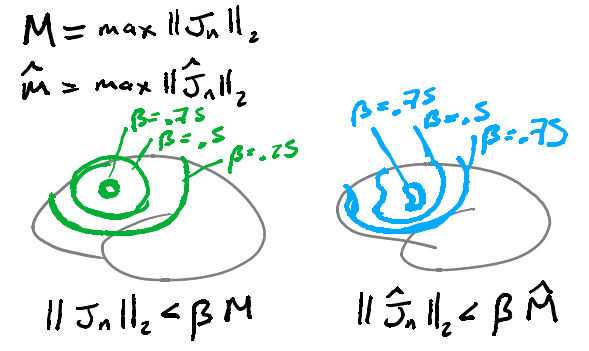
\includegraphics[width=0.8\linewidth]{./img_dev/nsCurves1}
%
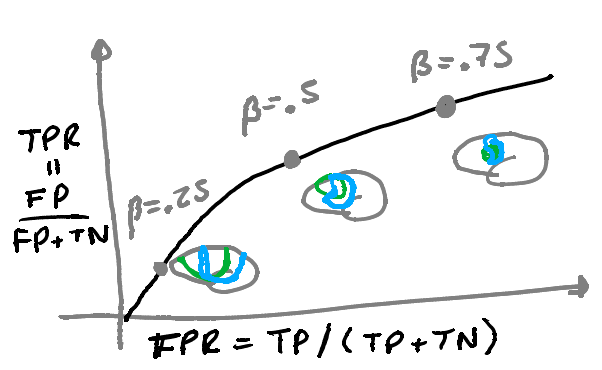
\includegraphics[width=0.4\linewidth]{./img_dev/nsCurves2}
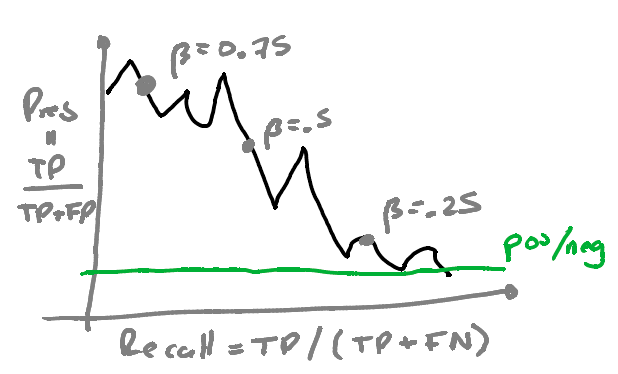
\includegraphics[width=0.4\linewidth]{./img_dev/nsCurves3}
\caption{Construction of Receiver-Operator Curve and Precision-Recall Curve from the reference and estimated dipole magnitudes, $\nnorm{{\J}}_2$ and $\nnorm{\hat{\J}}_2$, respectively.}
\end{figure}

The interpretation of the Receiver-Operator Curve is that each selection of $\beta$ balances the ratios of True Positives and False Negatives:
\begin{itemize}
\item 
Using a large $\beta$ will cause the labels to be strict, with very few False Positives but many False Negatives.
\item
Using a small $\beta$ will cause the labels to be permissive, with very few False Negatives but many False Positives.
\end{itemize}
In general, extreme values of $\beta$ will lead to the endpoints (0,0) and (1,1) of the ROC, and a somewhat smooth trajectory will be observed as $\beta$ increases.

A classifier for which TPR$(\beta)$ and $1-$FPR$(\beta)$ are close to 1 for all $\beta$'s is preferable, and this phenomenon can be observed in the ROC as being `close to the top'.
%
This concept is formalized by taking the are under the Area Under ROC (AUROC) is defined as the area under the ROC curve, being AUROC$\approx 1$ preferable.
%
In practice, the AUROC can be computed numerically using the trapezoid rule as follows
\begin{equation}
\text{AUROC}_\text{global} =
\frac{1}{2}
\sum_{i}
\ppar{ \text{FPR}\ppar{\beta_i}-\text{FPR}\ppar{\beta_{i-1}} }
\ppar{ \text{TPR}\ppar{\beta_i}+\text{TPR}\ppar{\beta_{i-1}} }
\end{equation}
with $\beta_i$ the finite number of values that $\beta$ can actually take.

The suffix `global' is added since all the dipoles are used in the computation of AUROC.
%
Some authors proposed that the AUROC value may be imprecise due to the severe class imbalance, i.e. we expect the proportion of active dipoles at any moment to be very low.
%
In order to alleviate that, they propose to use dipoles within certain distance to the true center.
%
We refer to that metric as $\text{AUROC}_\text{local}$, and use the distance as 5 \si{mm}.

\begin{figure}
\centering
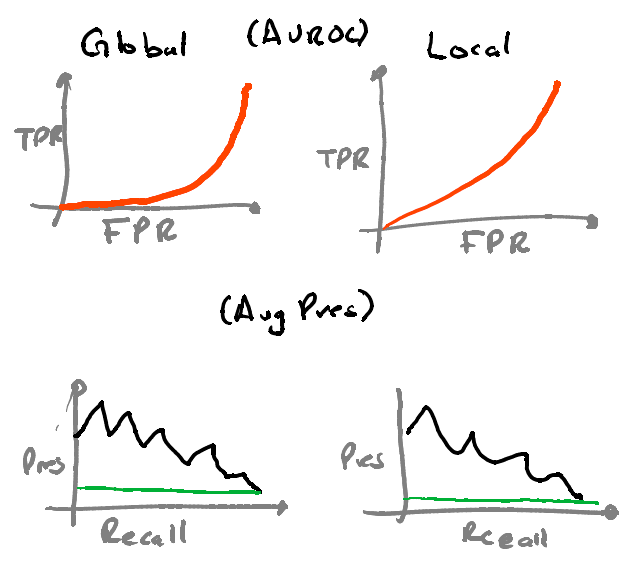
\includegraphics[width=0.8\linewidth]{./img_dev/nsCurves4}
\caption{Effect of neighborhood radius over the Receiver-Operator Curve and the Precision-Recall Curve. In order to attenuate the effects of class imbalance on the active/non-active dipoles, a small neighborhood around the source patch center is considered for the construction of the Receiver-Operator Curve and the Precision-Recall Curve, and in turn to compute the AUROC and Average Precision.}
\end{figure}

\subsection{Average Precision}

A different approach to the class imbalance of the AUROC is to use instead a quantity that is robust to this issue.

Average Precision, also known as Area Under Precision-Recall Curve, is based on the parametric curve 
$\ppar{\text{Rec}\ppar{\beta}, \text{Pre}\ppar{\beta}}$, with the Precision (Pre) and Rec (Rec) defined as
\begin{align}
\text{Precision}
&=
\frac{ \text{TP}\ppar{\beta} }{\text{TP}\ppar{\beta} + \text{FP}\ppar{\beta}}
\\
\text{Rec}
&=
\frac{ \text{TP}\ppar{\beta} }{\text{TP}\ppar{\beta} + \text{FP}\ppar{\beta}}
\end{align}

Similar to AUROC, Average Precision can be computed numerically as follows
\begin{equation}
\text{AUROC}_\text{global} =
\frac{1}{2}
\sum_{i}
\ppar{ \text{FPR}\ppar{\beta_i}-\text{FPR}\ppar{\beta_{i-1}} }
\ppar{ \text{TPR}\ppar{\beta_i}+\text{TPR}\ppar{\beta_{i-1}} }
\end{equation}

The characteristic shape of the Prcision-Recall Curve is quite different. 
%
For instance, see FIGURE.

%%%%%%%%%%%%%%%%%%%%%%%%%%%%%%%%%%%%%%%%%%%%%%%%%%%%%%%%
%%%%%%%%%%%%%%%%%%%%%%%%%%%%%%%%%%%%%%%%%%%%%%%%%%%%%%%%

\section{Numerical experiments}

In order to illustrate the characteristics and performance of the methods described in this section, those methods are first used over synthetic data.

The anatomical data is obtained from the ICBM 152 template[], which was constructed as an `average' of a T1 MRI scans from a number of different subjects.
%
Segmentation and surface extraction was omitted since the 4-sphere surfaces are provided.
%
Those triangulates surfaces are displayed in figure \ref{fig:surfaces}.

\begin{figure}
\centering
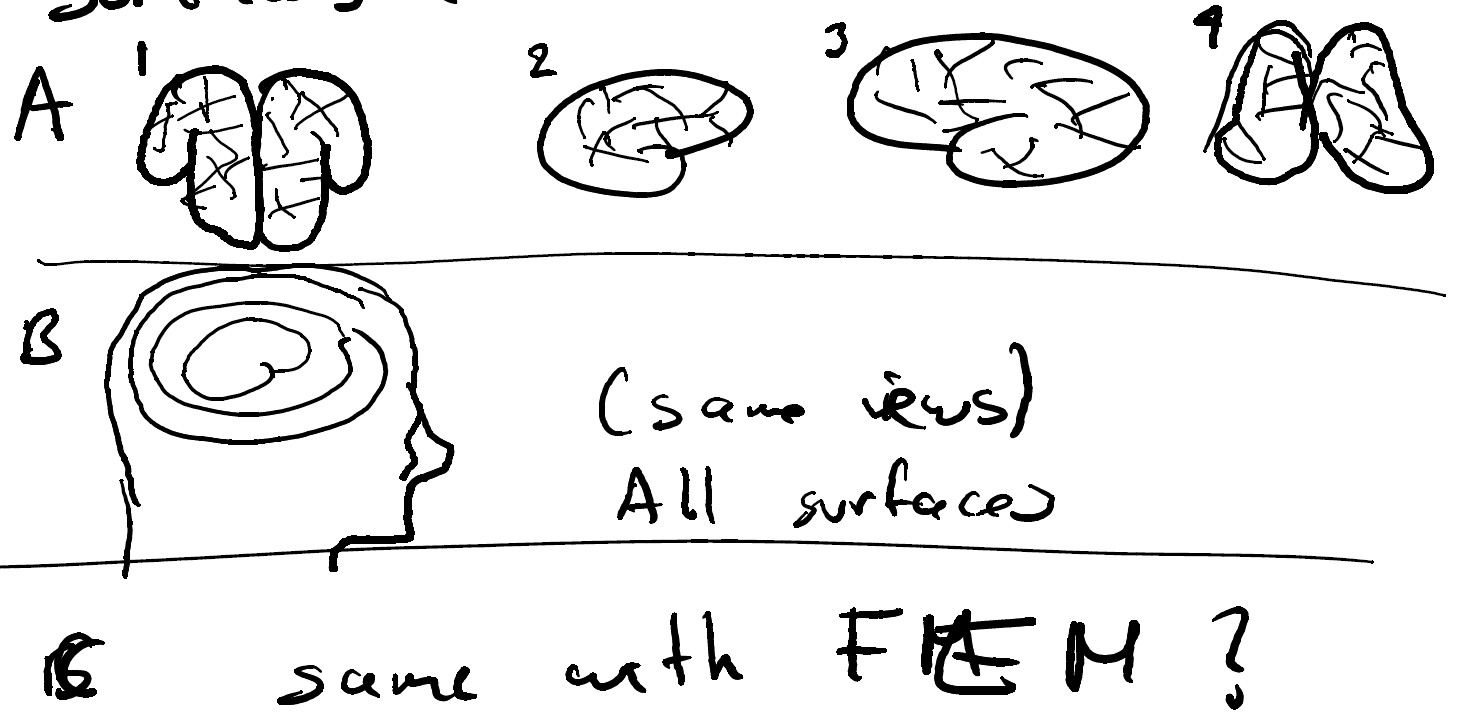
\includegraphics[width=0.8\linewidth]{./img_dev/nsSetupForward}
\caption{A. Cortex surface for the ICBM 152 template, consisting on 15,002 vertices. Views from top, left, right, back. B. Triangulated surfaces used for the 4-sphere forward model: cortex, inner skull, outer skull, head.}
\label{fig:surfaces}
\end{figure}

Electrodes were placed according to the 10-10 International System [], resulting on a total of $M=90$ electrodes. See either figure \ref{fig:1010system} for visual reference or [] for a more precise description of the electrode placement protocol.
%
The electrodes would be re-referenced to average, so no reference electrode is considered at this stage.

Dipole locations were determined using the $N=15,002$ available in triangulated cortex surface.
%
Dipole orientations were assumed to be orthogonal to the cortex surface.

Additionally, for illustrative purposes in this section, only a single time-stamp is considered, i.e. $T=1$.

\begin{figure}
\centering
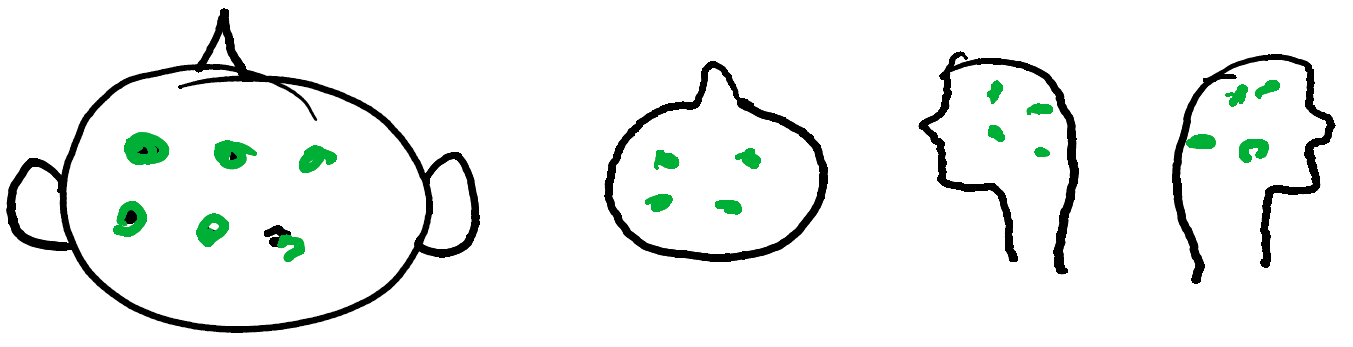
\includegraphics[width=0.8\linewidth]{./img_dev/nsElectrodeSetup}
\caption{Electrode Placement according to the 10-10 International System.}
\label{fig:1010system}
\end{figure}

%\subsubsection{Synthetic data protocol}

Following the forward model from equation \eqref{eq:general}, the synthetic data is constructed by (1) constructing $\J$ based on a source distrubition described later, then (2) constructing $\nu$ and $\varepsilon$ to meet a prescriped Signal-to-Noise Ratio (SNR), and finally (3) constructing $\Y$ as in the forward model.

The source distribution consist on selecting an arbitrary dipole indexed by $n^*$, and then construct $J$ as
\begin{equation}
\J_n = f\ppar{ \nnorm{r_n-r_{n^*}} / \kappa }
\end{equation}
with $f:\R_+\rightarrow \R_+$ a decreasing function and $\kappa>0$ a scaling parameters.
%
See figure \ref{fig:exaple_true} for a representation of the location and extent of the extended source.

\begin{figure}
\centering
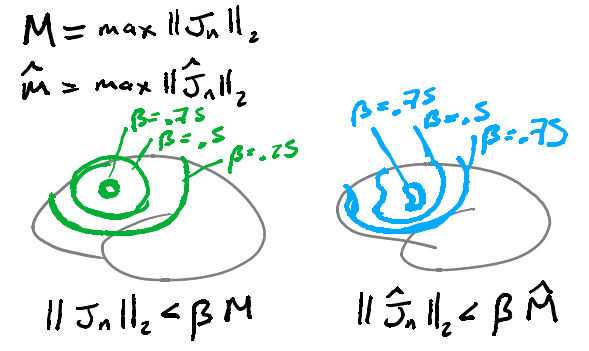
\includegraphics[width=0.8\linewidth]{./img_dev/nsCurves1}
\caption{Cortical patch used for creation of synthetic data.}
\label{fig:exaple_true}
\end{figure}

This type of configuration is referred to as `source patches' or `extended sources', since they occupy an area that is too large to be modeled as a single dipole.

For the synthetic data in this section, the dipole $n^*$ was selected within the frontal cortex for visibility.
%
We use 
\begin{equation}
f(x) = \begin{cases}
1, &\text{if } x\leq 1 \\
0, &\text{otherwise}.
\end{cases}
\end{equation}
and $\kappa = $ 12.6 \si{mm}, so to obtain a source patch with an area of 5 \si{cm^2} approximately.

For simplicity within the model formulation, we considered no internal noise ($\nu=0$) and independent gaussian noise at the sensors, i.e. $\varepsilon_m \sim\norm\ppar{0, \sigma_m^2}$ for $m = 1, \dots, M$ for some parameters $\sigma_m\geq 0$.
%
Under these conditions, the distribution of $\Y$ is given by
\begin{equation}
\ppar{\Y \given \J} =
\norm\ppar{ \G\, \J, \diag{\sigma_1, \dots, \sigma_M}^2 }
\end{equation}

The channel SNR (in dB) for the $m-th$ sensor is given by
\begin{equation}
\text{SNR}_m = 
10\, \log\ppar{ \frac{ \ppar{ \spar{\G\, \J}(m)}^2 }{\sigma_m^2} }
\end{equation}
With a prescribed SNR value, the parameters $\sigma_m$ are selected as follows
\begin{equation}
\sigma_m = 
\spar{\G\, \J}(m)\,
10\wedge \ppar{-\frac{SNR}{10}}
\end{equation}

For the synthetic data in this section we consider a SNR level of 20 dB, which we considered a low-noise condition.


%%%%%%%%%%%%%%%%%%%%%%%%%%%%%%%%%%%%%%%%%%%%%%%%%%%%%%%%
%%%%%%%%%%%%%%%%%%%%%%%%%%%%%%%%%%%%%%%%%%%%%%%%%%%%%%%%

%\section{Multi-modal asymmetric methods}
%
%A common framework
%to enhance ESI is to incorporate 
%`information' from the additional {modalities} of data:
%%and then constrain ESI to it.
%%
%%Multiple authors have explored the idea 
%%of enhancing 
%%the EEG Source Localization
%%by adding data from other `modes' of data: 
%MEG, MRI/fMRI\cite{he2008multimodal, huster2012methods}, PET, fNIRS\cite{fnirs}, etc.
%(Figure based on \cite{he2008multimodal}).
%%of using additional data to aid the EEG Source Localization, would it be MEG.
%\begin{figure}
%\centering
%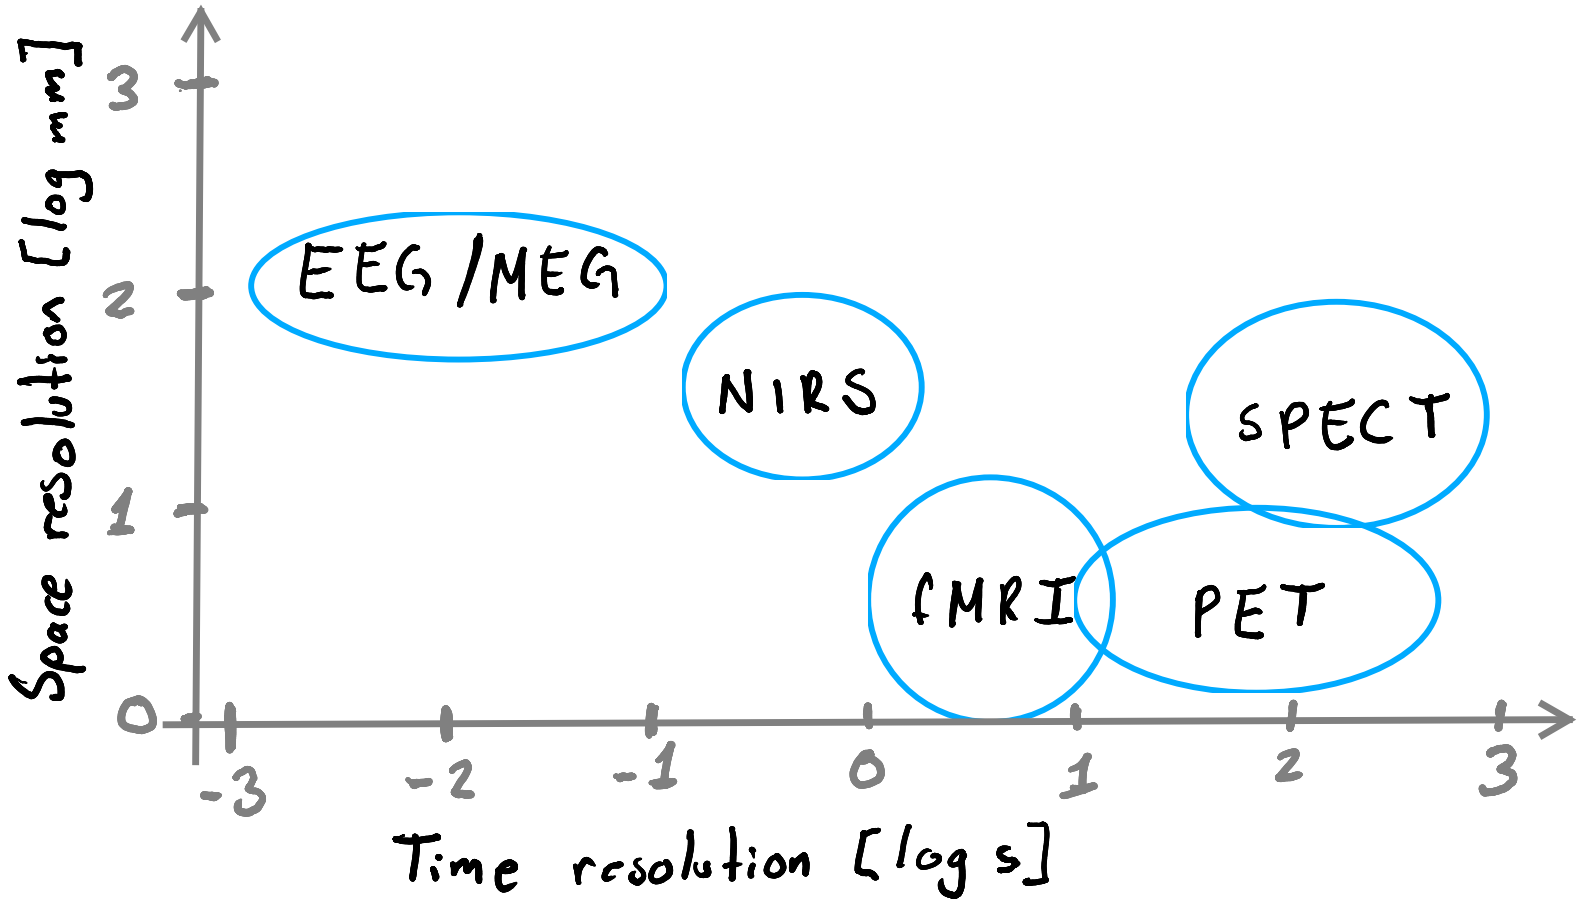
\includegraphics[width=0.65\linewidth]{./img_final/sketch07}
%\caption{PET=Positron Emission Tomography, NIRS=Near Infrared Spectroscopy, SPECT=Single-Photon Emission Computed Tomography}
%\end{figure}
%
%
%One big conceptual challenge for multimodal data integration is to model the interaction of the underlying physical phenomena. 
%%
%Focusing only on unilateral interactions results in asymmetric data integration.
%
%%For
%%asymmetric data integration, 
%%such as enhanced ESI, 
%%some bilateral interactions may be simplified. 
%%Thus 
%
%{Asymmetric data fusion} is the extraction of some parameters from one modality, which then are used to further the analysis of the other modality.
%%
%For ESI, the obtained parameters are typically used within the penalty functions.
%%Some simplifying assumptions considered in the literature for asymmetric data fusion for ESI are:
%%A common framework
%%Some techniques used in the literature 
%%to ESI enhancing is to extract `information' from the additional modalities and then constrain ESI to it.
%Some of the parameters extracted include:
%\begin{itemize}
%    \item Correlation networks
%    \item Statistical Parametric Maps (SPM)
%    \item Hidden activation variables \cite{fire}
%\end{itemize}

